%%% Template originaly created by Karol Kozioł (mail@karol-koziol.net) and modified for ShareLaTeX use

\documentclass[a4paper,11pt]{article}

\usepackage[T1]{fontenc}
\usepackage[utf8]{inputenc}
\usepackage{graphicx}
\usepackage{xcolor}
\usepackage[]{authblk}
\usepackage{subcaption}
\usepackage{multirow}

\renewcommand\familydefault{\sfdefault}
\usepackage{tgheros}
\usepackage[defaultmono]{droidmono}

\usepackage{amsmath,amssymb,amsthm,textcomp}
\usepackage{enumerate}
\usepackage{multicol}
\usepackage{tikz}

\usepackage{geometry}
%\geometry{total={210mm,297mm},
%left=25mm,right=25mm,%
%bindingoffset=0mm, top=20mm,bottom=20mm}


\linespread{1.2}

\newcommand{\linia}{\rule{\linewidth}{0.5pt}}

% custom theorems if needed
\newtheoremstyle{mytheor}
    {1ex}{1ex}{\normalfont}{0pt}{\scshape}{.}{1ex}
    {{\thmname{#1 }}{\thmnumber{#2}}{\thmnote{ (#3)}}}

%\theoremstyle{mytheor}
%\newtheorem{defi}{Definition}

% my own titles
\makeatletter
\renewcommand{\maketitle}{
\begin{center}
\vspace{1ex}
{\LARGE \textsc{\@title}}
\vspace{0.5ex}
\linia\\
\@author \hfill \@date
%\@personNumber \hfill \@email
\vspace{3ex}
\end{center}
}
\makeatother
%%%

% custom footers and headers
\usepackage{fancyhdr}
\pagestyle{fancy}
\lhead{}
\chead{}
\rhead{}
\lfoot{HW 4}
\cfoot{}
\rfoot{Page \thepage}
\renewcommand{\headrulewidth}{0pt}
\renewcommand{\footrulewidth}{0pt}
%

% code listing settings
\usepackage{listings}
\lstset{
    language=Python,
    basicstyle=\ttfamily\small,
    aboveskip={1.0\baselineskip},
    belowskip={1.0\baselineskip},
    columns=fixed,
    extendedchars=true,
    breaklines=true,
    tabsize=4,
    prebreak=\raisebox{0ex}[0ex][0ex]{\ensuremath{\hookleftarrow}},
    frame=lines,
    showtabs=false,
    showspaces=false,
    showstringspaces=false,
    keywordstyle=\color[rgb]{0.627,0.126,0.941},
    commentstyle=\color[rgb]{0.133,0.545,0.133},
    stringstyle=\color[rgb]{01,0,0},
    numbers=left,
    numberstyle=\small,
    stepnumber=1,
    numbersep=10pt,
    captionpos=t,
    escapeinside={\%*}{*)}
}

%%%----------%%%----------%%%----------%%%----------%%%

\begin{document}

\title{Hw 4: Autoencoders for Image Classification}

\author{Avinash Kommineni, 50248877} 
%\personNumber{50248877}
%\email{akommineni@buffalo.edu}
%\personNumber {50248877}
%\email{akommineni@buffalo.edu}
\date{\today}

\maketitle

\section*{Questions}

\subsection*{Q1. How does an autoencoder detect errors?}
The goal of an autoencoder is to induce a representation (encoding) for a set of data by learning an approximation of the identity function of this data. They work by combining data and try compressing it into features. These features are used to try reproduce the original image and the network is trained based on how accurately it is being able to regenerate the image. Any kind of error function can be used. Mean squared error is the default one used in MATLAB.

\subsection*{Q2. The network starts out with 28 × 28 = 784 inputs. Why do subsequent layers have fewer nodes?}
As the name indicates, the first part of autoencoders in encoding of the input and figure out underlying structure of the dataset. If the number of nodes in the hidden layer is equal to the 784, then the autoencoder is basically operating as an identity function and whereas if it is greater than 784, then the problem of overfitting comes into play as there is an oppurtunity of storing the data. Since the purpose of the network in encoding, i.e., combine data and try compressing it into features, the number of nodes in the hidden layer should be less than the input layer.\\
Sparsity contrainsts need to be applied if there a higher hidden layer nodes.

\subsection*{Q3. Why are autoencoders trained one hidden layer at a time?}
Each layer (apart from input layer) are generated such that they are able to reproduce its own input layer. So each layer of the autoencoders are trained separately.

\subsection*{Q4. How were the features in Figure 3 obtained? Compare the method of identifying features here with the method of HW1. What are a few pros and cons of these methods?}
We have a predefined filter bank in HW1 at multiple scales and colours. That is not same case here, as the features are automatically learned from the training data. The features encoded in the hidden layers in the process of learning in the autoencoder contains stroke patterns, edges and curls from the input images. Each node in the hidden layer has weights associated to it which are tuned during the training process and are activated/fired when the particular feature is experienced in the image. Features in an autoencoder change completely if the training dataset is different but the filter bank is same across all datasets for HW1.

\subsection*{Q5. What does the function plotconfusion do?}
It plots a confusion matrix between the ground truth and the predicted value.

\subsection*{Q6. What activation function is used in the hidden layers of the MATLAB tutorial?}
The activation function used in the MATLAB example tutorial is the default logistic sigmoid function defined by...
\begin{equation}
f (z) = \frac{1}{1+e^{-z}}
\end{equation}

\subsection*{Q7. In training deep networks, the ReLU activation function is generally preferred to the sigmoid activation function. Why might this be the case?}
There are several reasons why ReLU is preferred over Sigmoid activation function. Few of them areas follows...
\begin{itemize}
	\item It was found that ReLU greatly accelerate the convergence of stochastic gradient descent compared to the sigmoid functions. It is argued that this is due to its linear, non-saturating form.
	\item Compared to sigmoid neurons that involve expensive operations (exponentials, etc.), the ReLU can be implemented by simply thresholding a matrix of activations at zero.
	\item Sigmoids saturate and kill gradients. A very undesirable property of the sigmoid neuron is that when the neuron’s activation saturates at either tail of 0 or 1, the gradient at these regions is almost zero.
	\item Sigmoid outputs are not zero-centered. This is undesirable since neurons in later layers of processing in a Neural Network (more on this soon) would be receiving data that is not zero-centered.
\end{itemize}

\subsection*{Q8.}
Initializing a network with all zeros is not a good because if every neuron in the network computes the same output, then they will also all compute the same gradients during backpropagation and undergo the exact same parameter updates. In other words, there is no source of asymmetry between neurons if their weights are initialized to be the same.\\

Although initializing the network with all ones or some constant value doesn't have the same effect, it is recommended that the weights be initiialised to small values around 0 and a very small value for biases too so that the ReLU is activated from the beginning and therefore obtain and propagate some gradient.

\subsection*{Q9. Pros and cons for both stochastic and batch gradient descent}
\begin{itemize}
	\item Gradient Descent
		\begin{enumerate}
			\item Pros:
			 	\begin{itemize}
			 		\item It gives a gradient in the actual required direction.
			 		\item Since all of the input data is considered in calculating the gradient, it is more accurate.
			 	\end{itemize}
		 	\item Cons:
		 	\begin{itemize}
		 		\item If the dataset is huge, like in the order of few GigaBytes to TeraBytes, all of this data cannot be loaded into the memory (RAM) for each step.
		 		\item Which, even if possible is a huge computational expense and time consuming.
		 	\end{itemize}
		\end{enumerate}
	\item Stochastic Gradient Descent
	\begin{enumerate}
		\item Pros:
		\begin{itemize}
			\item Since only one example is considered for each step, the computation is fast and time effecient.
			\item SGD proves to be very handy if the dimensionality and the dataset sizes are big.
		\end{itemize}
		\item Cons:
		\begin{itemize}
			\item Since only one example is considered at every step, the gradient with respect to that particular example need not be in the right direction.
			\item The gradient might most probably take some zig-zag pattern to reach the minima.
			\item Randomization is must for this to ensure that th
		\end{itemize}
	\end{enumerate}
	\item In terms of number of epochs, SGD achieves the minima faster than batch gradient descent. This is possible because the networks takes multiple steps for each epoch istead of just 1.
	\item In terms of number of iterations, batch gradient descent will achieve a better results for an n number of iterations because SGD is not accurate in predicting the gradient and batch is like a cumulative.
	\item Mini-batch gradient descent is something in between batch gradient descent and SGD.
\end{itemize}


\subsection*{Q10. Exploration}
\begin{itemize}
	\item 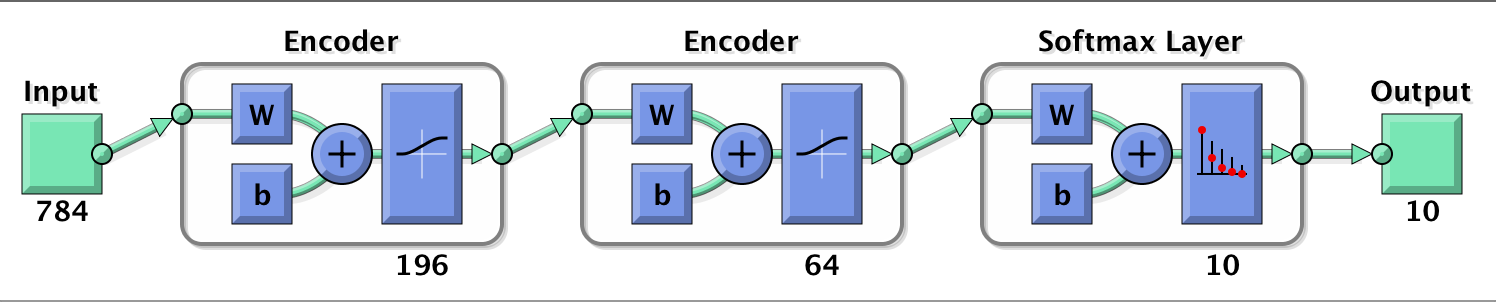
\includegraphics[scale=0.6]{3} \vfill
	\item Increasing the number of hidden layers increases the accuracy.
	\item With 100 hidden layers...\\ 
	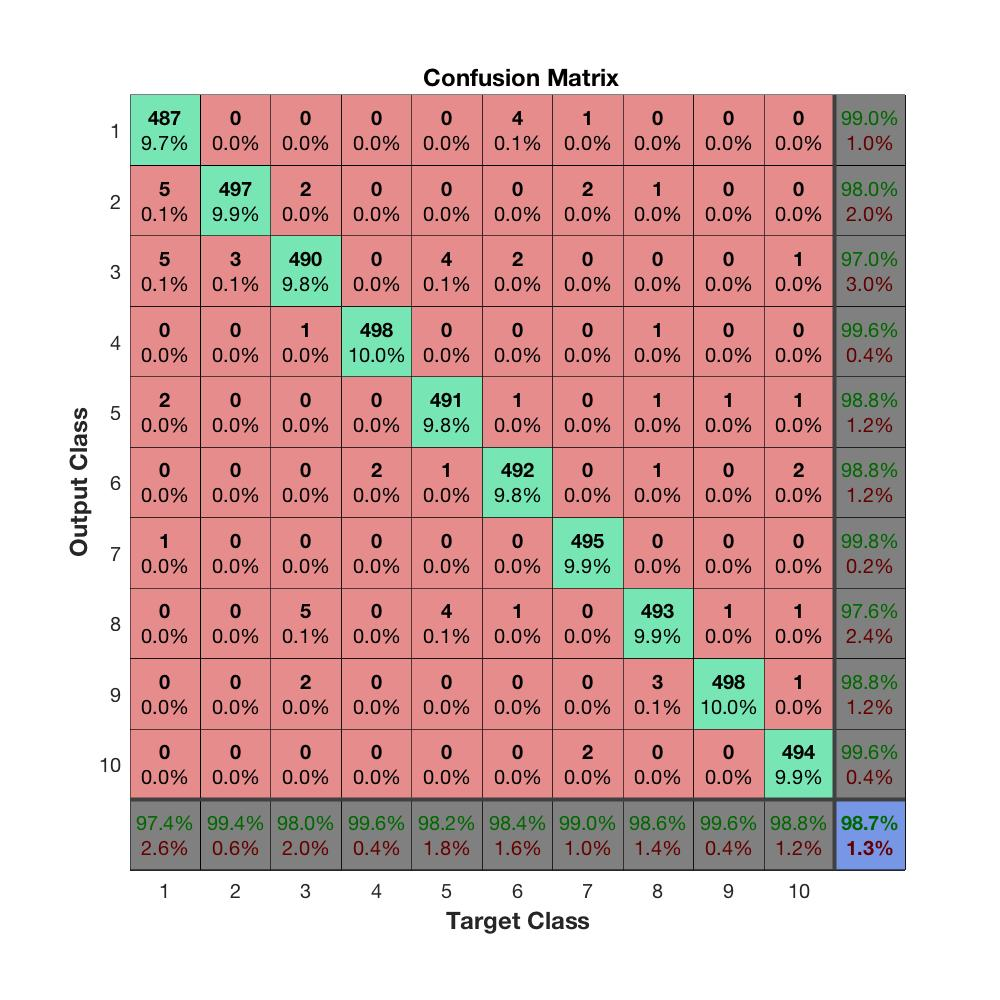
\includegraphics[scale=0.4]{1}\\ \vfill
	\item With 196 hidden layers...\\
	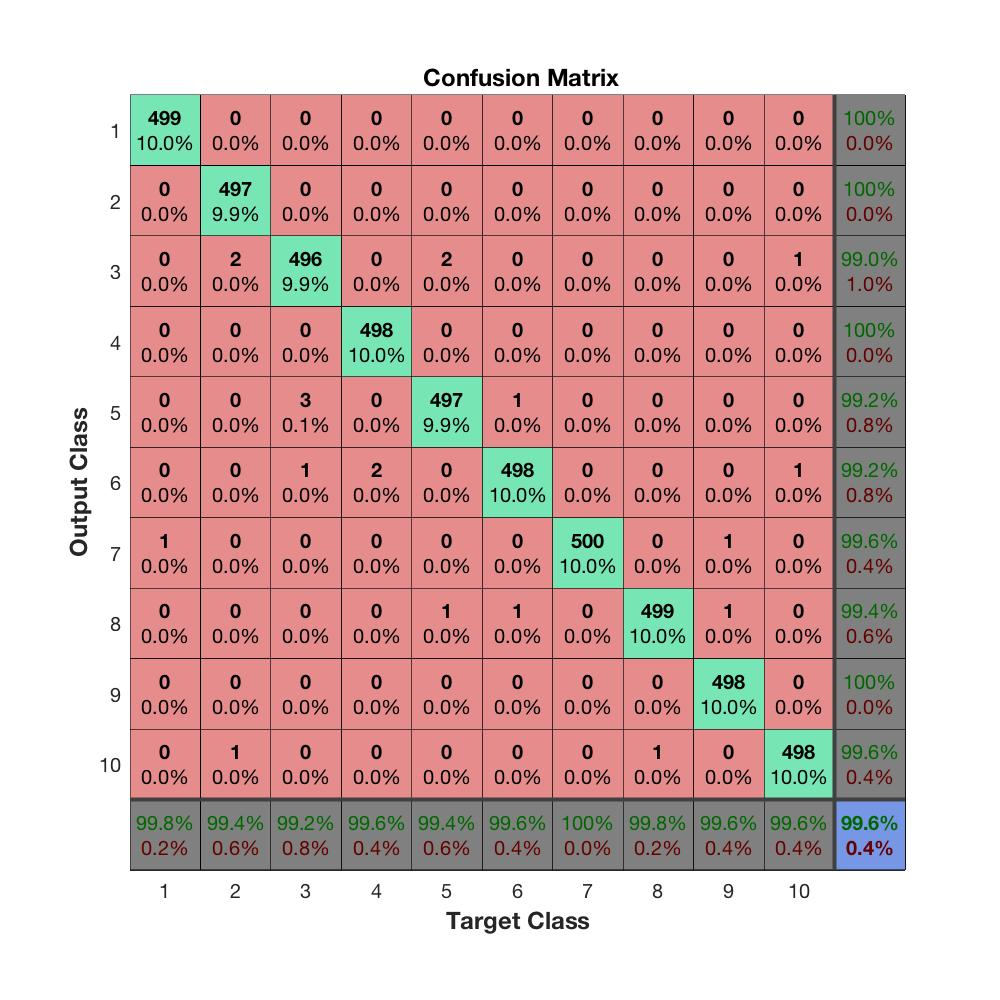
\includegraphics[scale=0.4]{2}
\end{itemize}

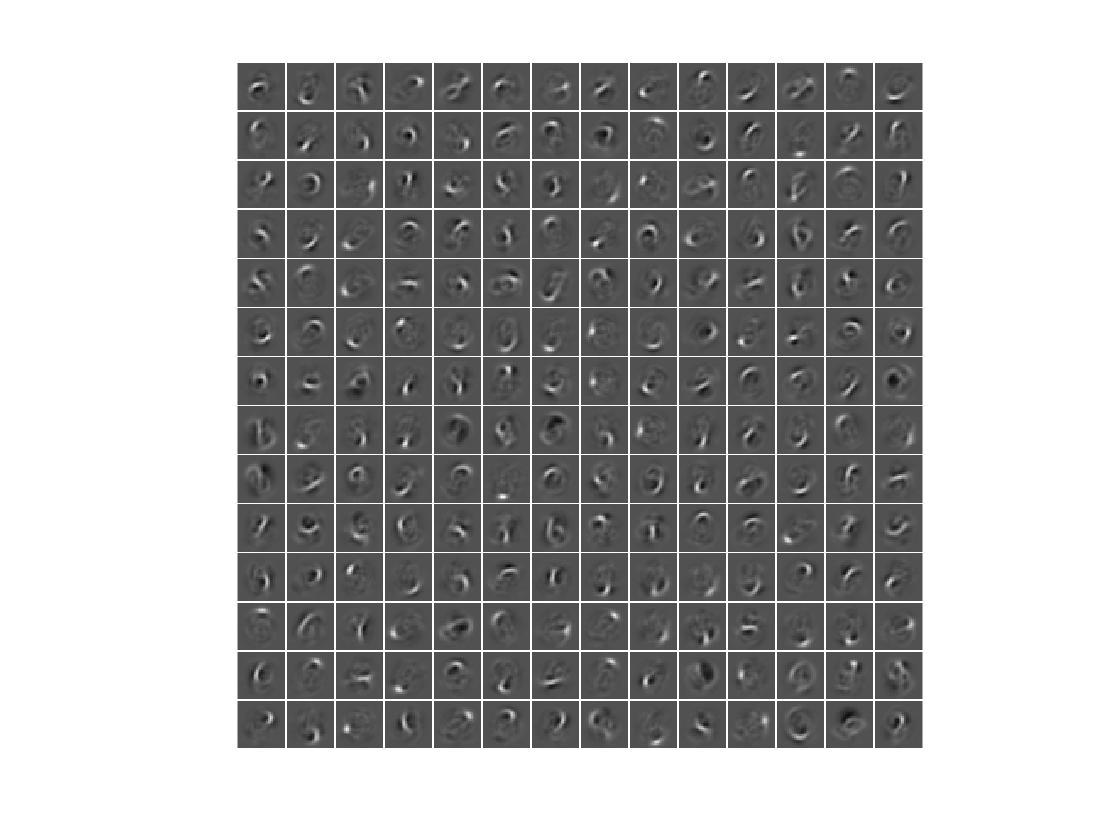
\includegraphics[scale=0.5]{4}\\


\vfill

\end{document}
